\documentclass{article}
\usepackage{graphicx}
\usepackage{enumerate}
\usepackage{amsmath}
\usepackage{mathtools}
\usepackage{float}
\usepackage{listings}
\usepackage{subfigure}
\usepackage{booktabs}
\usepackage{bm}
\usepackage{url}
\usepackage{appendix}
\usepackage{mathtools, nccmath}
\title{Time Series Research Project}
\author{Matej Rojec}
\date{June 26, 2023}

\begin{document}

\maketitle
\newpage

\tableofcontents
\listoffigures
\listoftables

\newpage

\begin{abstract}
    In the project we analysed the impact of different covariets to understand the impact of them to glycosolated hemoglobin and to diabetes. We conducted a thorough exploratory data analysis, we fitted a gamma regression model, interpreted the model. We concluded that the covariates that have the biggest impact on glycosolated hemoglobin and therefore diabetes are total cholesterol, stabilized glucose, age and waist length in inches.
\end{abstract}

\section{Modeling a time series of hourly-ground-levels of ozon}

\subsection{Introduction}

Ground-level ozone ($\text{O}_3$) is a type of air pollutant that occurs near the Earth's surface. It is not emitted directly into the atmosphere but is formed through complex chemical reactions between precursor pollutants in the presence of sunlight. The two primary precursor pollutants involved in the formation of ground-level ozone are nitrogen oxides ($\text{NO}_\text{x}$) and volatile organic compounds (VOCs).

NOx and VOCs are emitted from various sources, including vehicle emissions, industrial processes, power plants, and chemical solvents. When these pollutants are released into the atmosphere, they undergo chemical reactions in the presence of sunlight and react to form ground-level ozone.

Ground-level ozone is considered a harmful air pollutant and a significant component of smog. High concentrations of ozone can have adverse effects on human health, vegetation, and the environment. It can cause respiratory problems, exacerbate asthma, and contribute to lung inflammation. Ozone exposure can also harm plants, reduce crop yields, and damage ecosystems.

Monitoring and controlling ground-level ozone levels are essential for air quality management and public health protection. Ozone levels are typically monitored using ground-based monitoring stations that measure the concentration of ozone in the ambient air. This data is used to assess air quality, inform regulatory actions, and provide warnings to the public during periods of high ozone concentrations. \cite{i1}

Our task will be to fit a SARIMA-type model for five time series. The time series are hourly-ground-levels of $\text{O}3$ values, in micrograms per cubic meter ($\mu g/m^3$), collected in 2021 at the following five stations of the qualar network \cite{i2}:

\begin{itemize}
    \item Alfragide (Amadora)
    \item  Reboleira (Amadora)
    \item  Olivais (Lisboa)
    \item  Beato (Lisboa)
    \item  Entrecampos (Lisboa).
\end{itemize}


\subsection{Examination of the data}

The five data sets include 8760 rows each, one for each hour in the year 2021.
\subsubsection{Missing values, trend and seasonality}
Each of the five data sets has missing values. To cope with these values we will use the function \verb|na_interpolation| from the package \verb|imputeTS|  in \verb|R|. The function performs linear interpolation to fill in the missing values. Linear interpolation estimates missing values by assuming a straight line between the nearest non-missing values on either side of the missing value.

\begin{figure}[ht!]
   \centering
   \subfigure[Amadora ground-level ozone levels in 2021]{
   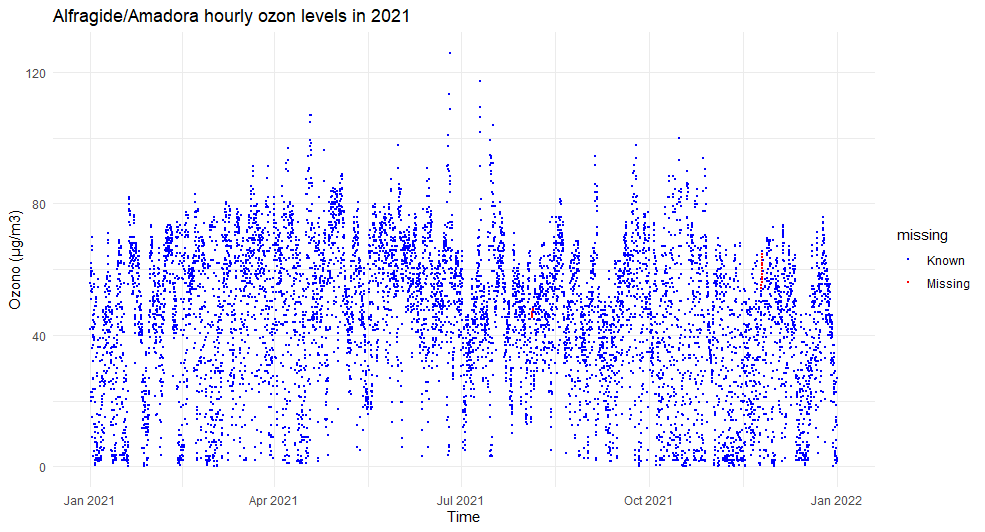
\includegraphics[width=0.45\textwidth]{Plots1/eda1.png}
   }
      \subfigure[Reboleira ground-level ozone levels in 2021]{
   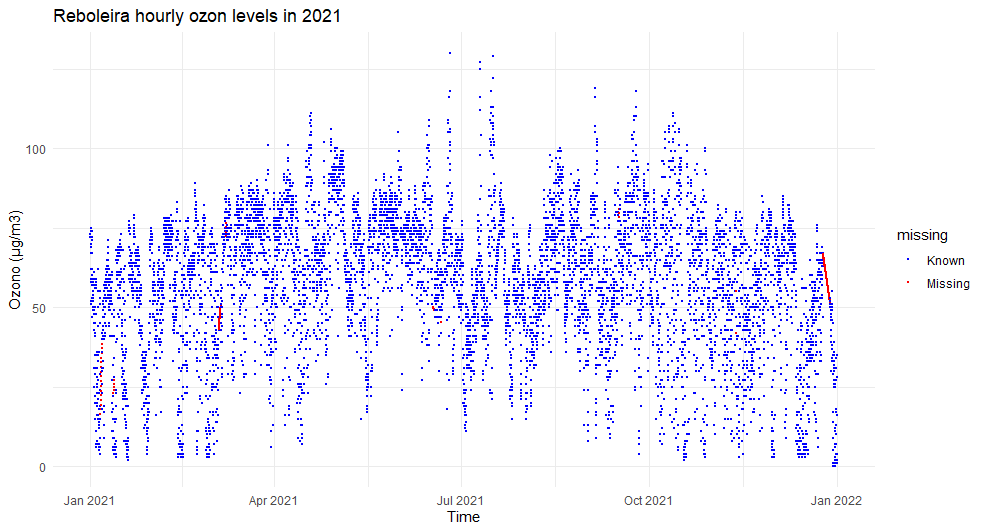
\includegraphics[width=0.45\textwidth]{Plots1/eda2.png}
   }
   \subfigure[Beato ground-level ozone levels in 2021]{
   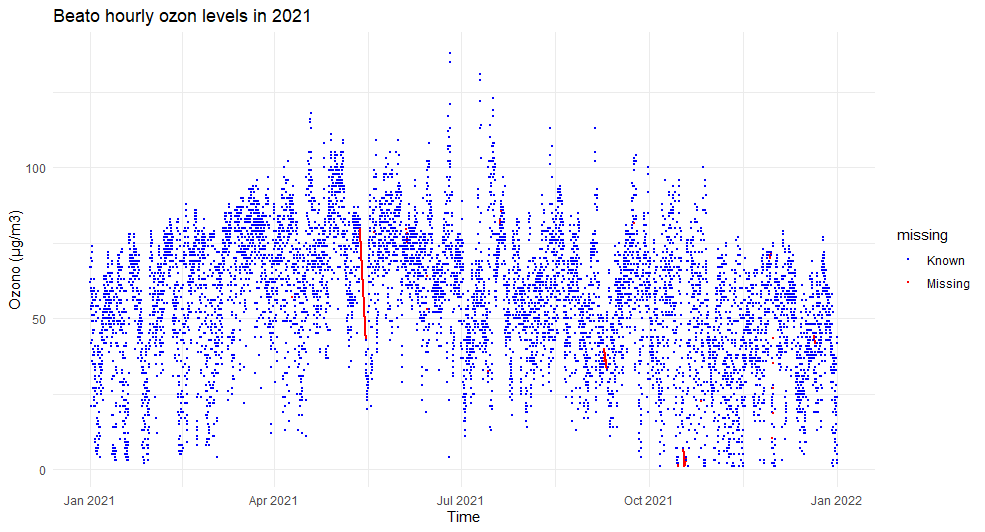
\includegraphics[width=0.45\textwidth]{Plots1/eda3.png}
   }
   \subfigure[Olivais ground-level ozone levels in 2021]{
   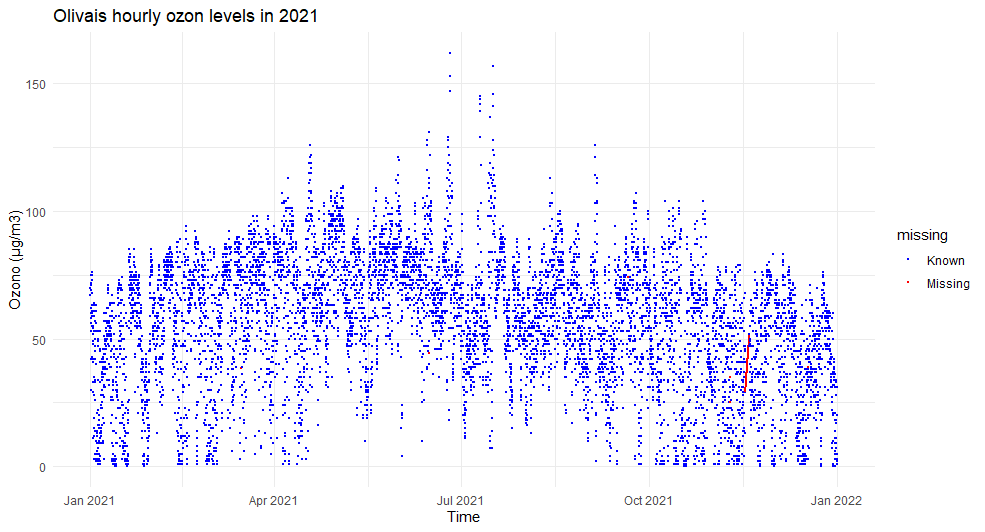
\includegraphics[width=0.45\textwidth]{Plots1/eda4.png}
   }
  \subfigure[Entrecampos ground-level ozone levels in 2021]{
   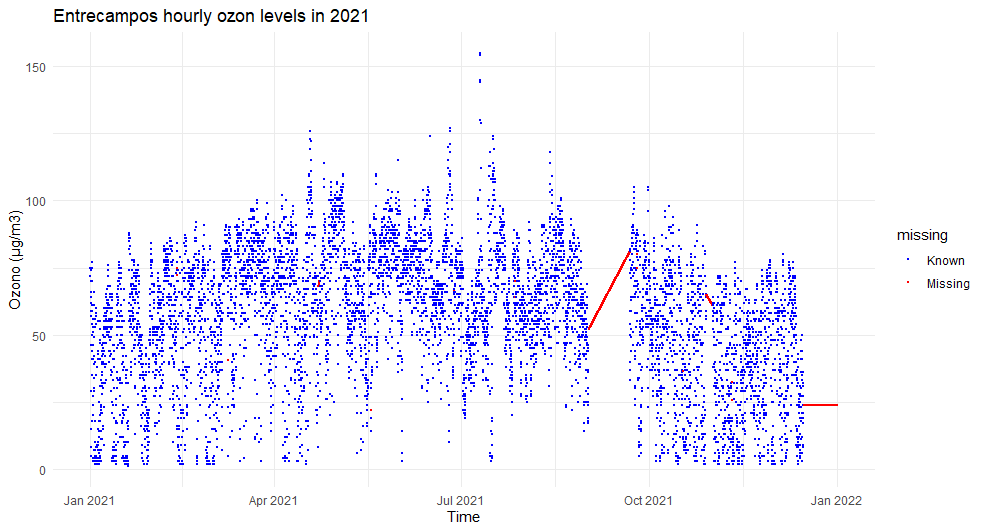
\includegraphics[width=0.45\textwidth]{Plots1/eda5.png}
   }
   \caption{Time series visualisations.}
    \label{fig:1}
\end{figure}

Figure \ref{fig:1} shows us the five time series and when there was missing data in the time series. It can be observed from figure \ref{fig:1} that Entrecampos has the most missing data.  Let's also look at the correlation between the different time series. We can see from table \ref{tab:correlation} that there seems to be a big correlation between the time series, especially between Beato and Olivais.

\begin{table}
  \centering
  \begin{tabular}{lccccc}
    & Alfragide\textbackslash Amadora & Reboleira & Entrecampos & Olivais & Beato \\
    \hline
    Alfragide \textbackslash Amadora & 1.00 & 0.85 & 0.81 & 0.87 & 0.86 \\
    Reboleira & 0.85 & 1.00 & 0.80 & 0.86 & 0.85 \\
    Entrecampos & 0.81 & 0.80 & 1.00 & 0.87 & 0.86 \\
    Olivais & 0.87 & 0.86 & 0.87 & 1.00 & 0.93 \\
    Beato & 0.86 & 0.85 & 0.86 & 0.93 & 1.00 \\
    \hline
  \end{tabular}
  \caption{Correlation matrix for the hourly-ground-levels of $\text{O}3$ time series.}
  \label{tab:correlation}
\end{table}

This correlation can be further supported by figure \ref{fig:2} that shows all the time series together in the first five days of 2021. The figure also shows that there is a daily periodicity in the data. From the figure we see that the means are not invariant with time. This implies that the time series are not stationary. 

\begin{figure}[ht!]
    \centering
    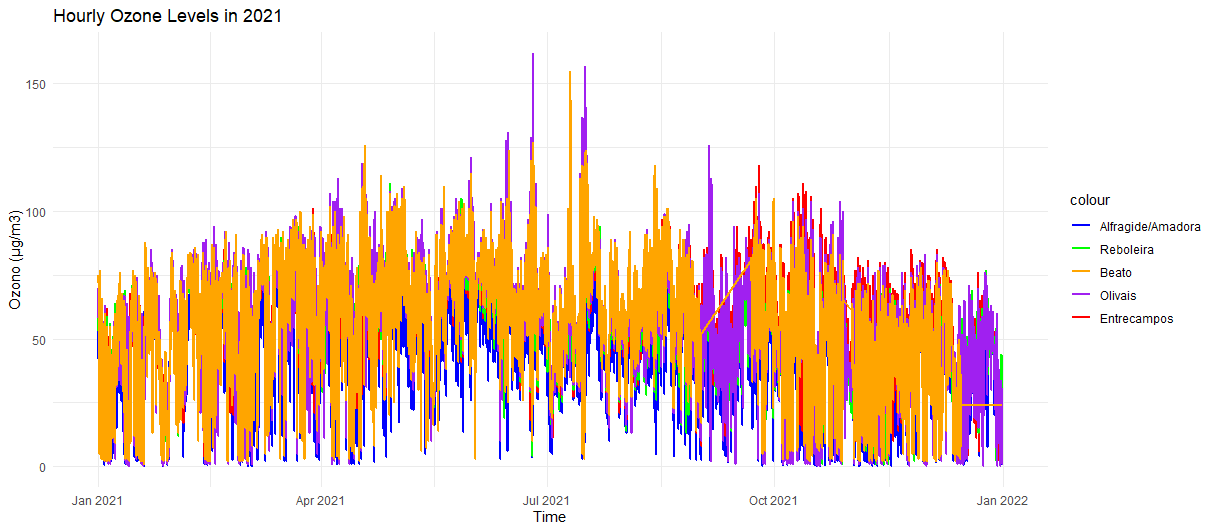
\includegraphics[width=0.95\textwidth]{Plots1/eda6.png}
    \caption{Comparison of the five time series of hourly-ground-levels of $\text{O}_3$ in the first five days of 2021.}
    \label{fig:2}
\end{figure}

Ozone levels often exhibit patterns due to various factors, including meteorological conditions, sunlight intensity, temperature, and the presence of precursor pollutants. In many regions, ozone levels tend to be higher during the summer months when there is increased sunlight and warmer temperatures. These conditions promote the formation of ozone through chemical reactions involving nitrogen oxides ($\text{NO}_\text{x}$) and volatile organic compounds (VOCs). This component can be observed in figure \ref{fig:1} in all five time series. There is also a daily seasonality in the data as seen from figure \ref{fig:2}. During the day there are higher levels of ozon and during the night there are lower levels of ozon. 

We can further analyse the seasonal-trend decomposition  with the help of the function \verb|STL| in \verb|R|. The decomposition for Alfragide can be seen on figure \ref{fig:std}. The figure further supports that there is a seasonal as well as a trend component to the data. The same conclusion follows for the other four time series. 

\begin{figure}[ht!]
    \centering
    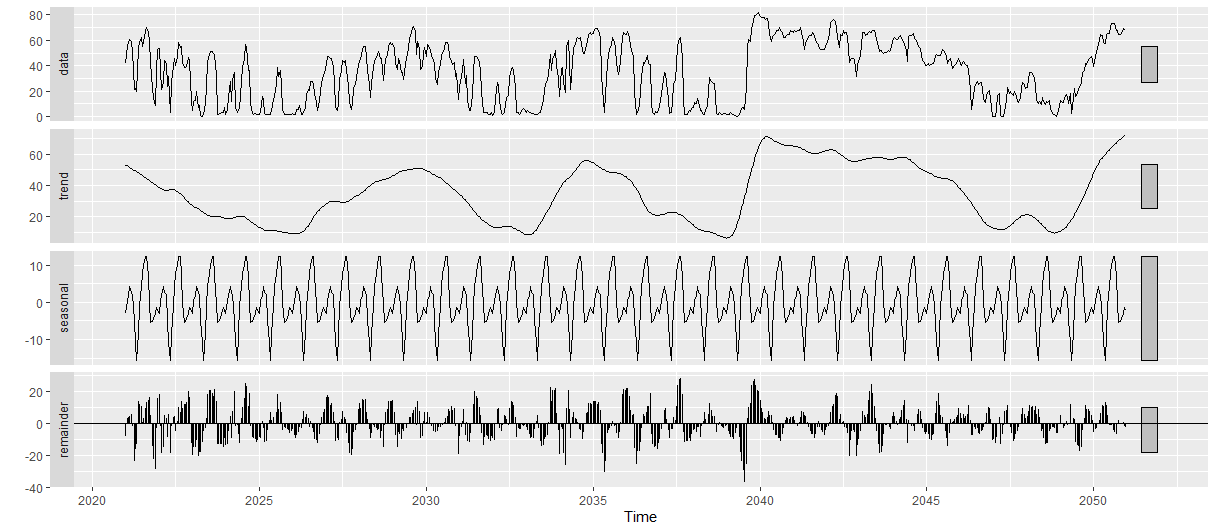
\includegraphics[width=0.80\textwidth]{Plots1/eda7.png}
    \caption{Seasonal-trend decomposition for Alfragide in the firt month of 2021.}
    \label{fig:std}
\end{figure}

From figure \ref{fig:1} we can notice times with higher and lower peaks. Therefor we need to stabilise the data with some sort of transformation to get a stationary time series. We will look at three possible transformations of the data:
\begin{enumerate}
    \item logarithmic transformation of the data;
    \item 24 hour seasonal difference transformation of the data;
    \item 24 hour seasonal and a 1 hour non-seasonal difference transformation of the data.
\end{enumerate}

The three time series can be seen in figure \ref{fig:ts_trans}. From them we can see that the  logarithmic transformation and the the 24 hour seasonal difference transformation of the data does not look like a stationary time series while the 24 hour seasonal and a 1 hour non-seasonal difference transformation of the data seems to resemble a stationary time series. 

\begin{figure}[ht!]
   \centering
   \subfigure[Logarithmic transformation of the data.]{
   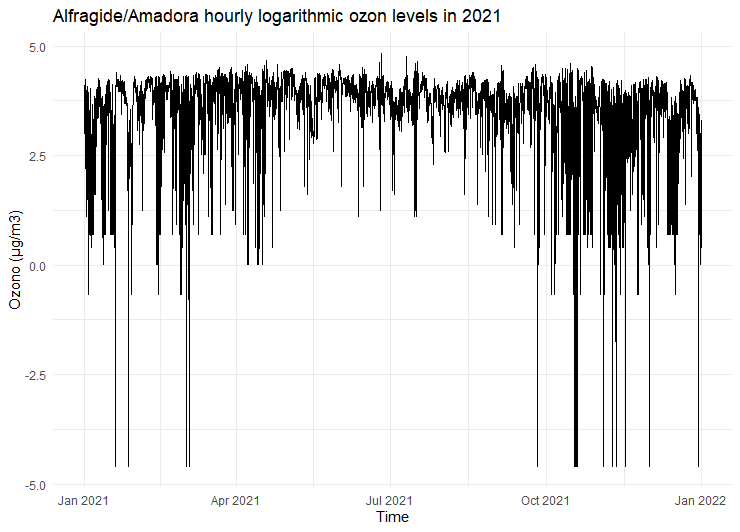
\includegraphics[width=0.3\textwidth]{Plots1/eda16.png}
   }
   \subfigure[24 hour seasonal difference transformation of the data.]{
   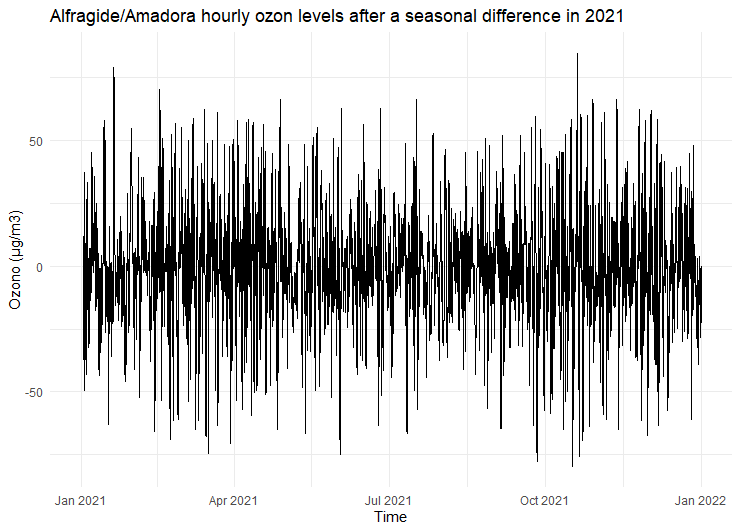
\includegraphics[width=0.3\textwidth]{Plots1/eda17.png}
   }
   \subfigure[24 hour seasonal and a 1 hour non-seasonal difference transformation of the data.]{
   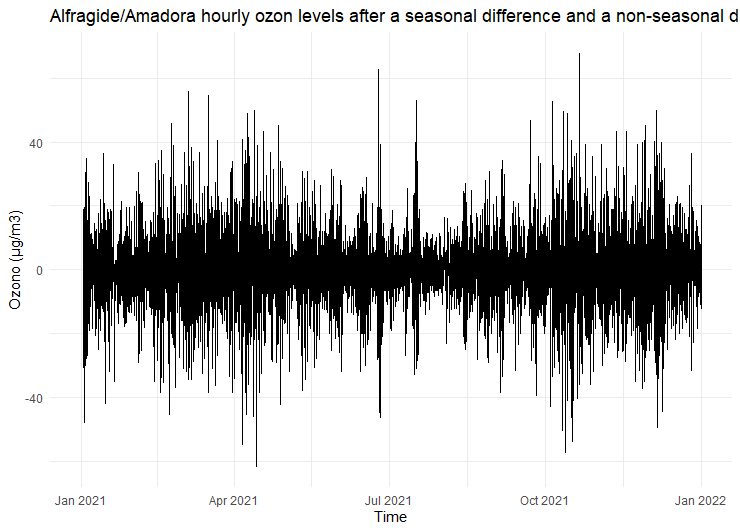
\includegraphics[width=0.3\textwidth]{Plots1/eda18.png}
   }
   \caption{Transformed time series data.}
    \label{fig:ts_trans}
\end{figure}




\subsection{The transformations and the initial dependence orders}
\label{ch:ea} 

Firstly let us look at the ACF and the PACF of the initial data and the log transformed data. The ACF, as seen from figures \ref{fig:acf} and \ref{fig:acflog}, for both the log transform and original data doesn’t exhibit the classic exponential drop to 0 displayed by clear \verb|AR(p)| processes. However, we do see a pattern that tends somewhat towards zero, but which may not be as clear-cut due to the daily seasonality we observed. In other words, the seasonality may be masking the exponential drop towards zero since
it shows up periodically in the ACF plot. 
%Nonetheless, we see that the PACF drops under the 95\% CI
%after $k = 2$ and $k =3$ for the original and the log transformed time series, respectively, which suggests
%an AR(1) model order for the non-seasonal component. 
In addition, we can see in both
PACFs that lags after the dashed lines (24 multiples) exceed the confidence bounds. This is in line
with our hypothesized daily seasonality. Note that immediately before the dashed lines, we also see
some lags that exceed the confidence bounds and slowly fade after 2 days of lag. This corresponds to the
last hours of the day (i.e. the evening) and potentially shows that there might be some correlation during those hours of the day across the board. 

If we look at the seasonally differentiated data in figure \ref{fig:acflagsez} we can see that ACF is decreasing to 0
faster, even though there are still spikes at multiples of 24. The PACF is more clear in this case with big spikes at multiples of 24.

If we look at the ACF and PACF data after a seasonal and a non-seasonal difference as seen in figure \ref{fig:acflagsezdof} we can notice that the time series seems stationary. Furthermore, the ACF and the PACF now behave as something that we can interpret. Specifically, the ACF shows a seasonal spike at lag 24 (as expected), and the PACF shows seasonal spikes at multiples of 24, which suggest a seasonal MA component.

In addition, we can see in both PACFs that lags after the dashed lines (24 multiples) exceed the confidence bounds. This is in line with our hypothesized daily seasonality. Even though the ACF doesn’t drop to 0 sufficiently fast as classical examples of \verb|AR(p)| processes, we suspect the daily periodicity maybe masking this and hence we move forward towards formulating our initial model.

Having this in consideration we can start with an initial model as \\
\verb|SARIMA|$(0,1,0) \times (1,1,0)_{24}$, since we see that the series is stationary and there with the seasonal and non-seasonal transformation. Another model we will consider as an initial model is \verb|SARIMA|$(0,0,0) \times (1,0,0)_{24}$ as we saw daily seasonality in the data. Further, to start with a model as simple as
possible, we can for now ignore any \verb|MA(q)| components in the initial model. 

\begin{figure}[ht!]
   \centering
   \subfigure[ACF  for the Alfragide data.]{
   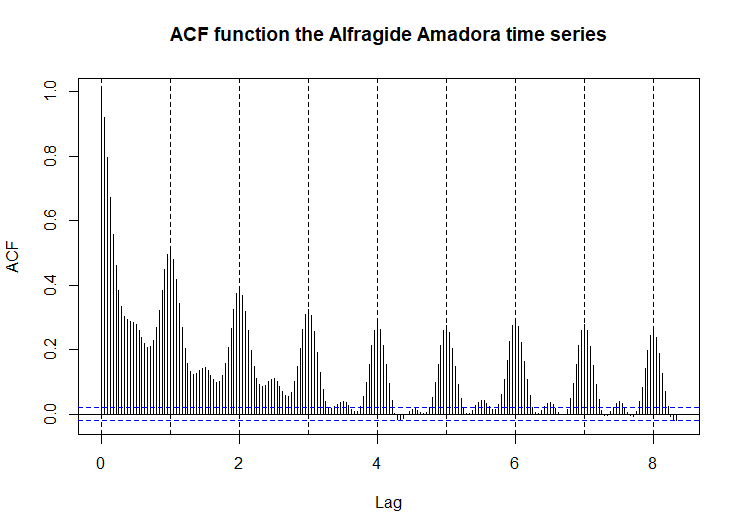
\includegraphics[width=0.4\textwidth]{Plots1/eda8.png}
   }
      \subfigure[ACF  for the log transformed Alfragide data.]{
   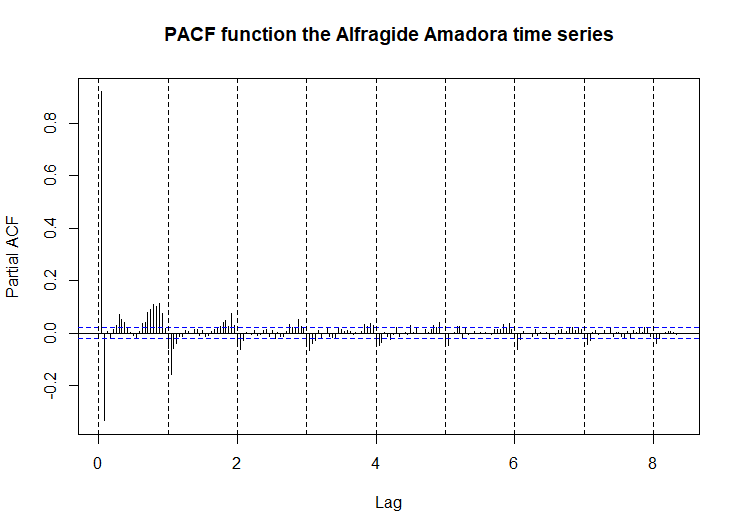
\includegraphics[width=0.4\textwidth]{Plots1/eda9.png}
   }
   \caption{ACF function for the Alfragide data.}
    \label{fig:acf}
\end{figure}

\begin{figure}[ht!]
   \centering
   \subfigure[PACF  for the Alfragide data.]{
   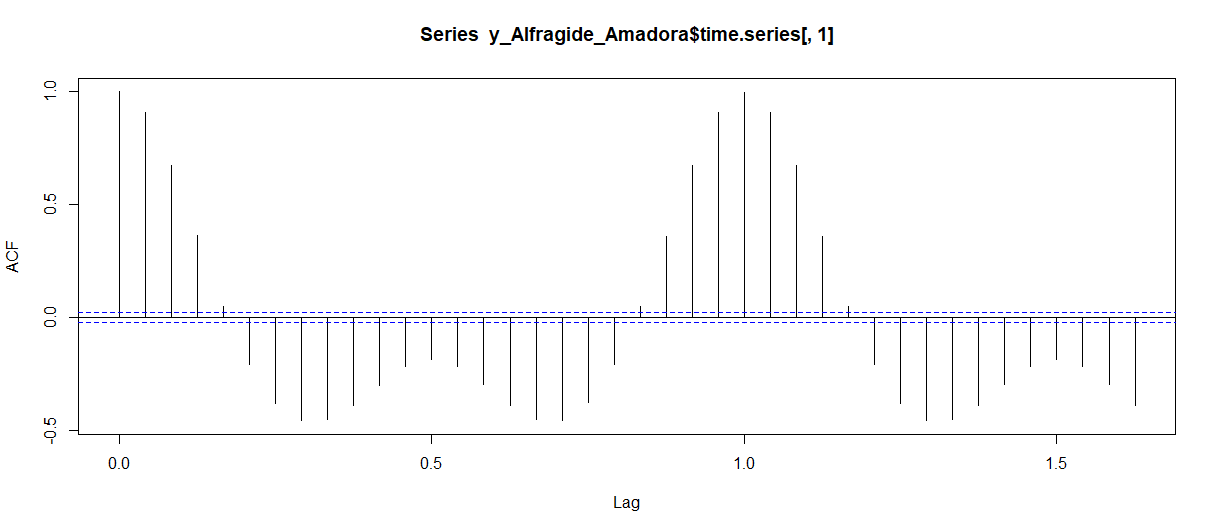
\includegraphics[width=0.4\textwidth]{Plots1/eda10.png}
   }
      \subfigure[PACF  for the log transformed Alfragide data]{
   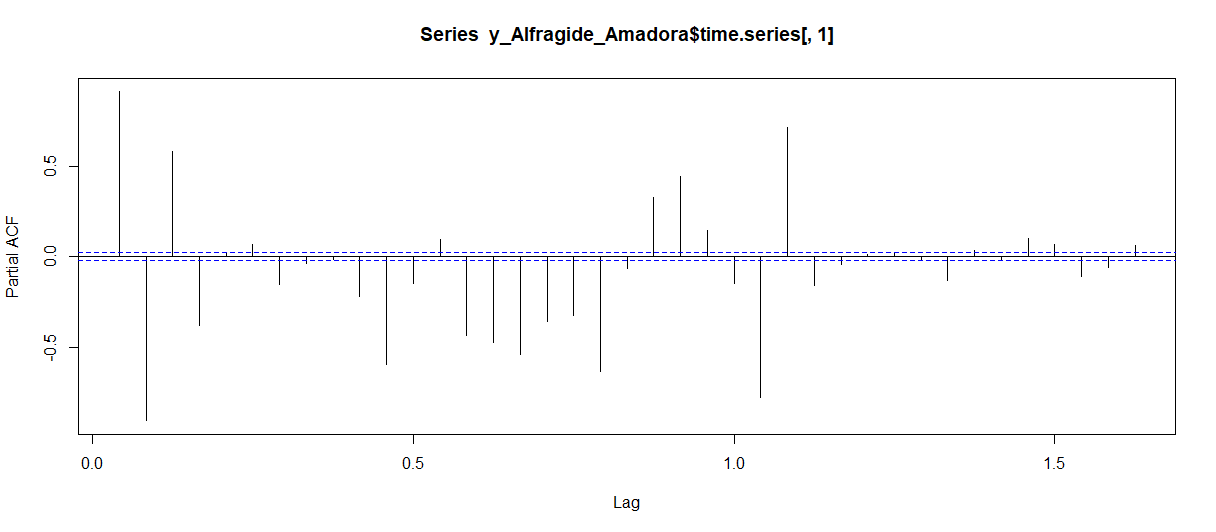
\includegraphics[width=0.4\textwidth]{Plots1/eda11.png}
   }
   \caption{ACF function for the log transformed Alfragide data.}
    \label{fig:acflog}
\end{figure}

\begin{figure}[ht!]
   \centering
   \subfigure[PACF for the seasonally differentiated  Alfragide data.]{
   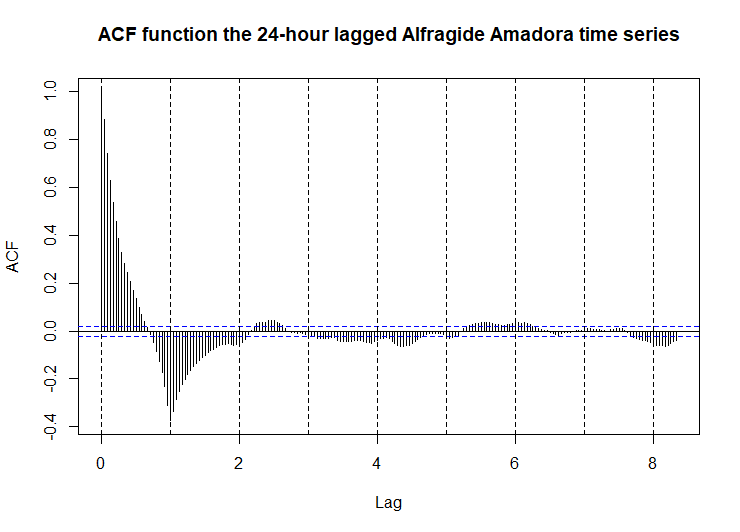
\includegraphics[width=0.4\textwidth]{Plots1/eda12.png}
   }
      \subfigure[PACF  for the seasonally differentiated  Alfragide data]{
   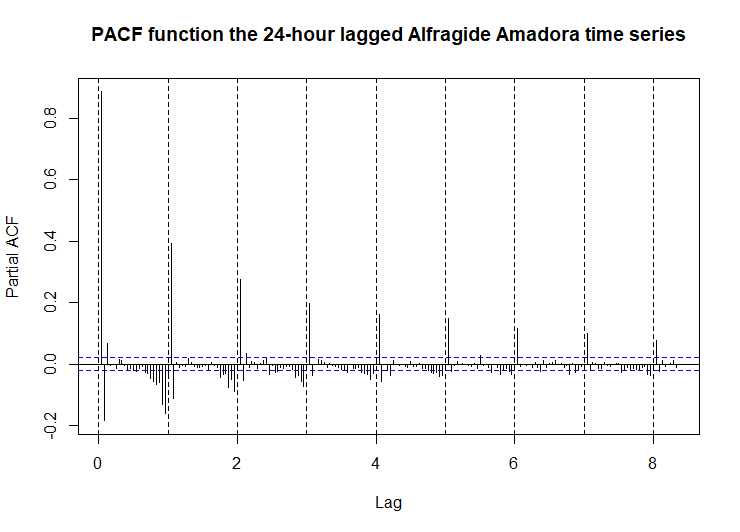
\includegraphics[width=0.4\textwidth]{Plots1/eda13.png}
   }
   \caption{ACF and PACF function for the seasonally differentiated Alfragide data.}
    \label{fig:acflagsez}
\end{figure}

\begin{figure}[ht!]
   \centering
   \subfigure[PACF for the seasonally differentiated and normally differentiated Alfragide data.]{
   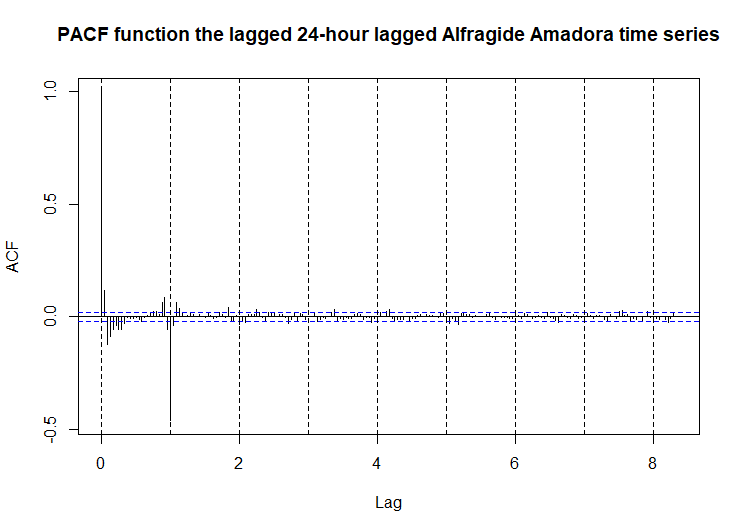
\includegraphics[width=0.4\textwidth]{Plots1/eda14.png}
   }
      \subfigure[PACF  for the seasonally differentiated and normally differentiated Alfragide data]{
   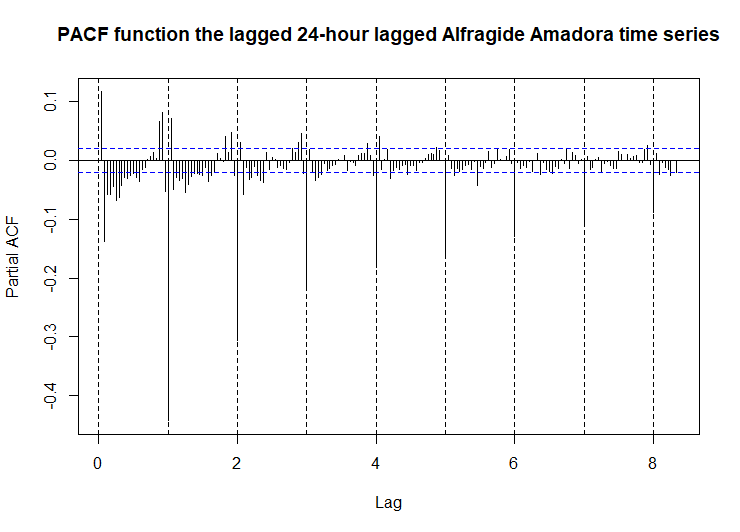
\includegraphics[width=0.4\textwidth]{Plots1/eda15.png}
   }
   \caption{ACF and PACF for the seasonally differentiated and normally differentiated Alfragide data.}
    \label{fig:acflagsezdof}
\end{figure}


\subsection{Model selection and residual diagnostics}

As discussed in chapter \ref{ch:ea} we can make two initial models to start with. Another model we will take as our initial model is the one produced by the function \verb|auto.arima| in \verb|R|. That being 
\verb|SARIMA|$(5,1,0) \times (2,0,0)_{24}$. So the three initial models are therfore:
\begin{enumerate}
    \item \verb|SARIMA|$(0,1,0) \times (1,1,0)_{24}$,
    \item \verb|SARIMA|$(0,0,0) \times (1,0,0)_{24}$.
    \item \verb|SARIMA|$(5,1,0) \times (2,0,0)_{24}$.
\end{enumerate}

From there on we will iterate through different models. We take the initial models above and try different variations of them and compare them (when relevant) using the AIC measure. However, we can only use AIC within models of the same seasonal
difference order. Therefore, we also compute the RMSE of each model to do cross-comparison across models of different seasonal difference orders. 

In table \ref{model:ozon} we can see the AIC and RMSE for the fitted models.

\begin{table}[htbp]
  \centering
  \begin{tabular}{lccccc}
    \toprule
    \textbf{Model} & \textbf{AIC} & \textbf{RMSE} \\
    \midrule
    \verb|SARIMA|$(0,1,0) \times (1,1,0)_{24}$&  63386 & 7.7 \\ \hline 
    \verb|SARIMA|$(0,0,0) \times (1,0,0)_{24}$  & 76182 & 18.7  \\ \hline
    \verb|SARIMA|$(5,1,0) \times (2,0,0)_{24}$ & 61144 & 7.9  \\ \hline
    \verb|SARIMA|$(1,0,1) \times (2,1,0)_{24}$ & 61722 & 8.3  \\ \hline
    \verb|SARIMA|$(3,0,1) \times (1,0,1)_{24}$ & 59934 & 7.4  \\ \hline
    \verb|SARIMA|$(3,0,0) \times (1,0,0)_{24}$ & 60834 & 7.8  \\ \hline
    \verb|SARIMA|$(1,0,1) \times (1,0,1)_{24}$ & 59931 & 7.4  \\ \hline
    \verb|SARIMA|$(2,0,1) \times (1,1,1)_{24}$ & 59781 & 7.4  \\ \hline
    \verb|SARIMA|$(2,1,1) \times (1,1,1)_{24}$ & 59812 & 7.4  \\ \hline
    \verb|SARIMA|$(1,0,1) \times (1,0,2)_{24}$ & 59931 & 7.4  \\ 
    \bottomrule
  \end{tabular}
  \caption{AIC and RMSE of the fitted models for the Alfragide ozon-ground level time series .}
  \label{model:ozon}
\end{table}

Model results can be found in table \ref{model:ozon} with the model with the lowest AIC and the lowest RMSE being \verb|SARIMA|$(2,0,1) \times (1,1,1)_{24}$.

Model results can be found in table \ref{model:ozon} with the model with the lowest AIC and the lowest RMSE being \verb|SARIMA|$(2,0,1) \times (1,1,1)_{24}$ and \verb|SARIMA|$(1,0,1) \times (1,1,1)_{24}$.

For estimation of parameters we have used the \verb|arima| function in \verb|R|.  The \verb|SARIMA|$(2,0,1) \times (1,1,1)_{24}$ model has the following parameters found 
in table \ref{par:ozon}. We see that the $p-$value of the parameter ar2 is very high leading to the 
conclusion that it is not important for the model. As such we will consider the model \verb|SARIMA|$(1,0,1) \times (1,1,1)_{24}$ instead.


\begin{table}[ht!]
    \centering
    \begin{tabular}{|c|c|c|c|c|c|c|} \hline
        Parameter / Value & ar1 & ar2 & ma1 & sar1 & sma1  \\ \hline
        Value & 0.8168 & 0.0542 & 0.2765 & 0.0680 & -0.9423  \\ \hline
        $p$-value & 0.0000 & 25.0836 & 0.0000 & 0.0000 & 0.0000  \\ \hline
    \end{tabular}
    \caption{The parameters and the $p$-values of the model SARIMA$(2,0,1) \times (1,1,1)_{24}$.}
    \label{par:ozon}
\end{table}


Let us now take a closer look at the model \verb|SARIMA|$(1,0,1) \times (1,1,1)_{24}$. The analysis of the residuals
can be seen on figure  \ref{fig:res_o}. From the figure it can be seen that the the standardized 
residuals are an i.i.d. sequence with mean zero and variance one. From the ACF we do not see any 
patterns of large values. This is also supported by the Ljung-Box test, since the $p$-values are quite large.


\begin{figure}[ht!]
    \centering
    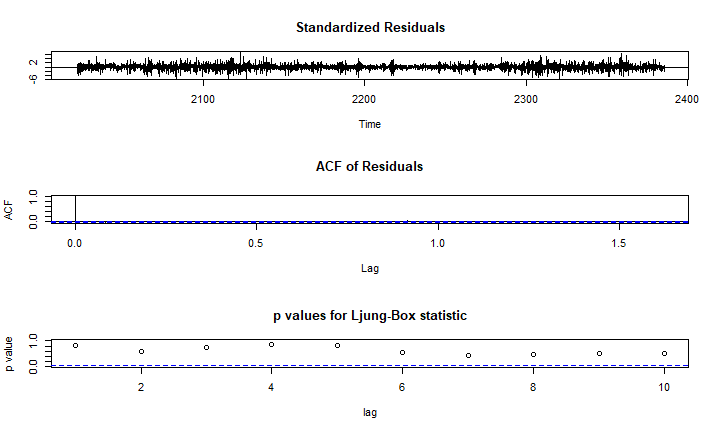
\includegraphics[width=0.95\textwidth]{Plots1/res_a.png}
    \caption{Residual analysis of the SARIMA$(1,0,1) \times (1,1,1)_{24}$.}
    \label{fig:res_o}
\end{figure}

Let's look also at the residual analysis of another model for comparison. Let's look at 
the model   \verb|SARIMA|$(3,0,0) \times (1,0,0)_{24}$. The residuals, as seen on 
figure \ref{fig:res_o2}, are also a i.i.d. sequence squance but the $p-$values for 
Ljung-Box statistic go to zero after lag 5, so that is why we prefer the first model.
If we look at the residual analysis of the other models we come to the same conclusion

\begin{figure}[ht!]
    \centering
    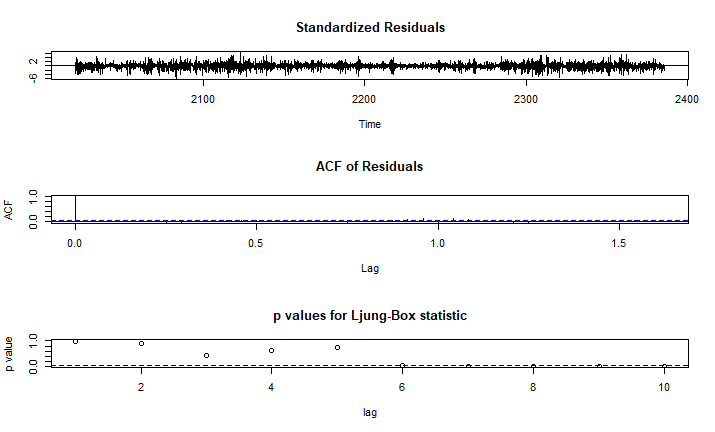
\includegraphics[width=0.95\textwidth]{Plots1/ra_2.png}
    \caption{Residual analysis of the SARIMA$(1,0,1) \times (1,1,1)_{24}$.}
    \label{fig:res_o2}
\end{figure}


For the other models we preform the same analysis. In table \ref{tab:final_ozon} we have the best 
model for each of the time series.

\begin{table}
    \centering
    \begin{tabular}{|l|c|}
        \hline
        Time Series & Model \\
        \hline
        Alfragide & SARIMA$(1,0,1) \times (1,1,1)_{24}$ \\
        \hline
        Reboleira & SARIMA$(3,0,1) \times (1,0,1)_{24}$  \\
        \hline
        Beato &   SARIMA$(1,0,1) \times (1,0,2)_{24}$ \\
        \hline
        Olivais &  SARIMA$(3,0,1) \times (1,0,1)_{24}$  \\
        \hline
        Entrecampos &  SARIMA$(1,0,1) \times (1,0,1)_{24}$ \\
        \hline
    \end{tabular}
    \caption{Final models for the five time series.}
    \label{tab:final_ozon}
\end{table}
    
\subsection{Prediction}

We have now decided on the appropriate models and now we will
forecast the data into the future up to 5 time periods
ahead and calculate 95\% prediction intervals for each of the 5 forecasts.

We will do this with the help of  \verb|R| with the function \verb|predict|.
From this we get predictions for five steps ahead and their 
respected standard errors. To get the 
95\% interval for each prediction we apply the following formula:
$$\text{CI}_{95} = [f - 2 \cdot \sigma, f + 2 \cdot \sigma],$$
where $\sigma$ is the standard errors of the forecasted value and 
$f$ is the forcasted value. 

The results for each of the five time series can be seen on figure 
\ref{fig:pred}. 

\begin{figure}[ht!]
    \centering
    \subfigure[Predicted and original hourly-ground-levels of ozon in Alfragide.]{
    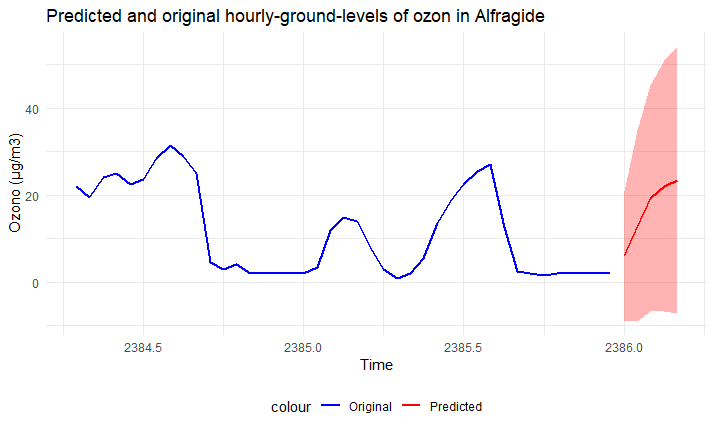
\includegraphics[width=0.45\textwidth]{Plots1/se1.png}
    }
       \subfigure[Predicted and original hourly-ground-levels of ozon in Reboleira.]{
    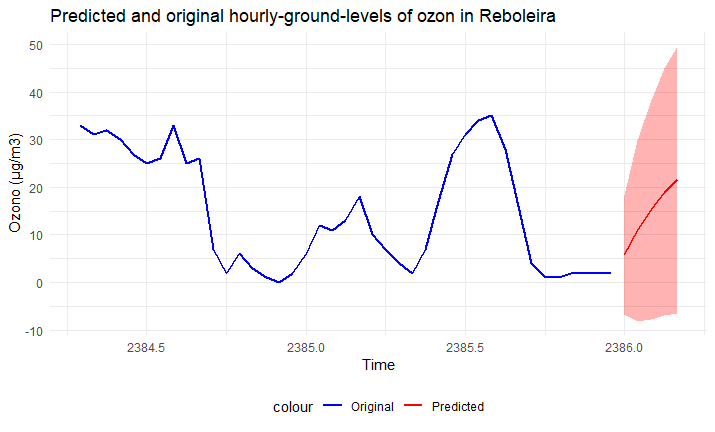
\includegraphics[width=0.45\textwidth]{Plots1/se2.png}
    }
    \subfigure[Predicted and original hourly-ground-levels of ozon in Beato.]{
    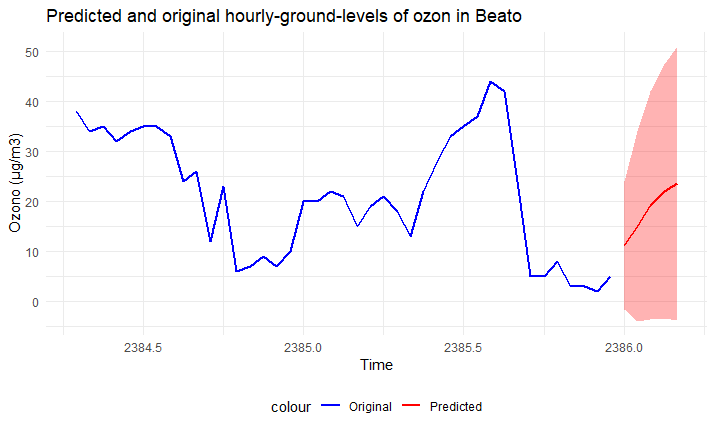
\includegraphics[width=0.45\textwidth]{Plots1/se3.png}
    }
    \subfigure[Predicted and original hourly-ground-levels of ozon in Olivais.]{
    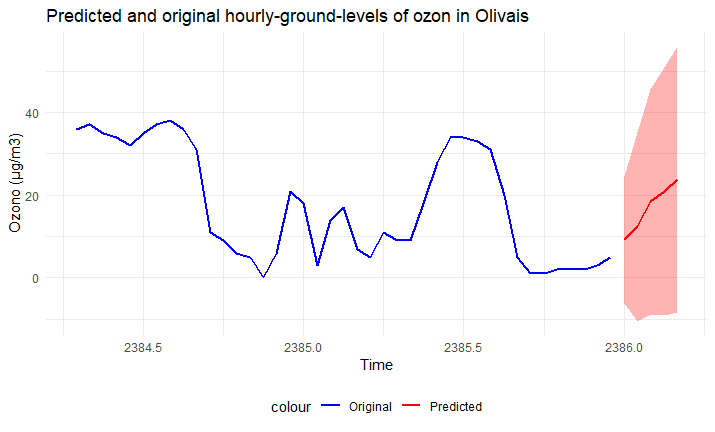
\includegraphics[width=0.45\textwidth]{Plots1/se4.png}
    }
   \subfigure[Predicted and original hourly-ground-levels of ozon in Entrecampos,]{
    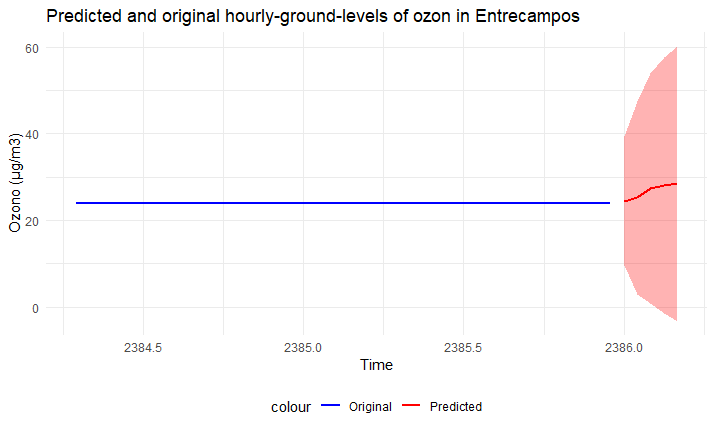
\includegraphics[width=0.45\textwidth]{Plots1/se5.png}
    }
    \caption{Time series visualisations.}
     \label{fig:pred}
 \end{figure}
 

\subsection{Conclusion}







\newpage

\section{Modeling a time series of hourly-ground-levels of log-returns}

\subsection{Introduction}

In finance, log returns are often used to measure the relative change in the price or value of a financial asset over a certain period of time. The log return of an asset is defined as the natural logarithm of the ratio of its price at time $t+1$ that is $P_{t+1}$  to its previous price at time $t$ that is $P_t$, expressed as a decimal or percentage.

The formula for log returns can be expressed as:

\begin{equation*}
\text{Log Return} = \ln \left(\frac{P_{t+1}}{P_t}\right).
\end{equation*}

Log returns provide several advantages, including the ability to simplify calculations involving asset returns and their statistical properties. Additionally, log returns can be added over time periods to obtain the cumulative log return.

We will be modeling five financial time series from 2022-01-05 to 2022-10-12 with the help of log returns, namely the daily share related-prices from five companies on Euronext Lisbon:  
\begin{itemize}
    \item Altri-SGPS,
    \item Mota Engil,
    \item Ren,
    \item Sonae,
    \item The Navigator Company.
\end{itemize} 
In our case the log returns will correspond to the daily closing prices.

\subsection{Examination of the data}
\label{sect:2.2}

The five data sets include 199 rows each, one for each day from 2022-01-05 to 2022-10-12 including the data: date, open, high, low, close, number of shares, number of trades, turnover and vwap. In our time series we will have 198 rows each containing the log returns corresponding to the daily closing prices and the date.
In the data there is no missing values so we do not need to interpolate. 

Figure \ref{fig:ts_lr} shows the log return of all five financial time series. 
We can calculate that the sample mean of the data is close to zero whereas the sample variance is of the order $10^{-4}$. From the figure \ref{fig:ts_lr} we can see that exceedances of high/low thresholds tend to occur in clusters. We can also conclude from the figure an asymmetric responses in the volatility.

\begin{figure}[ht!]
    \centering
    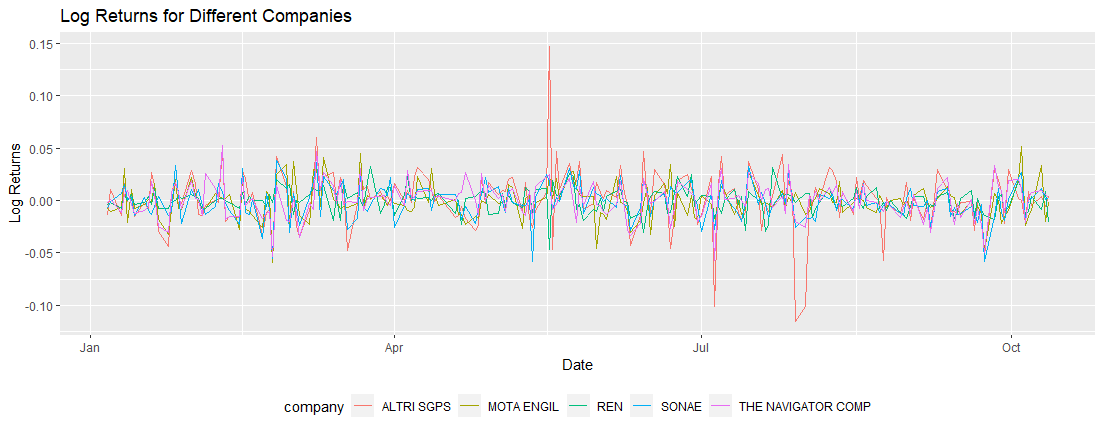
\includegraphics[width=0.95\textwidth]{Plots2/plot1.png}
    \caption{Time series of hourly-ground-levels of $\text{O}_3$ visualisation.}
    \label{fig:ts_lr}
\end{figure}

Let us now look at the ACF for all of the financial time series and the ACF of the squares of the time series. From figure
\ref{fig:acf_lr} we see that the sample ACF use to be negligible at all lags.  % From \ref{fig:acf_lr_sq} we can see that the sample ACF of the squares are different from zero for a large number of lags and stay almost constant and positive for large lags.

\begin{figure}[ht!]
   \centering
   \subfigure[The sample ACF for Altri-SGPS.]{
   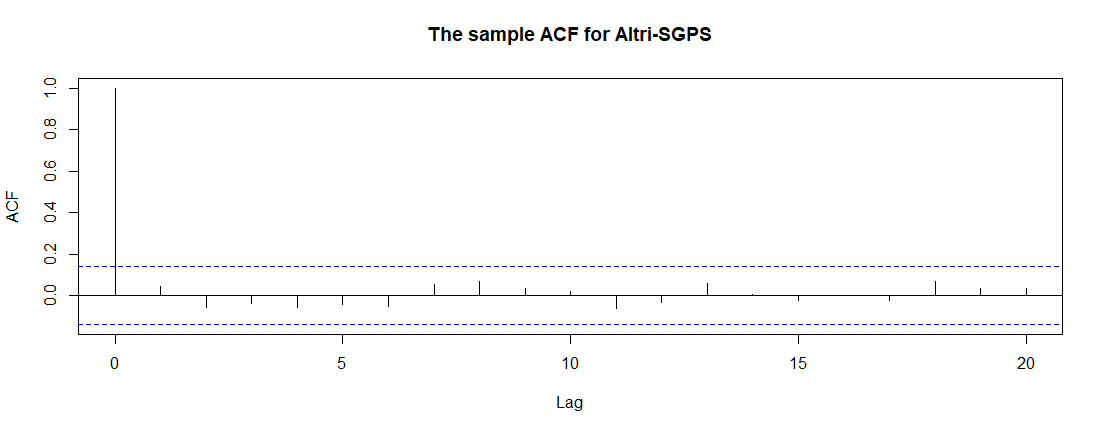
\includegraphics[width=0.45\textwidth]{Plots2/acf1.png}
   }
      \subfigure[The sample ACF for Mota Engil.]{
   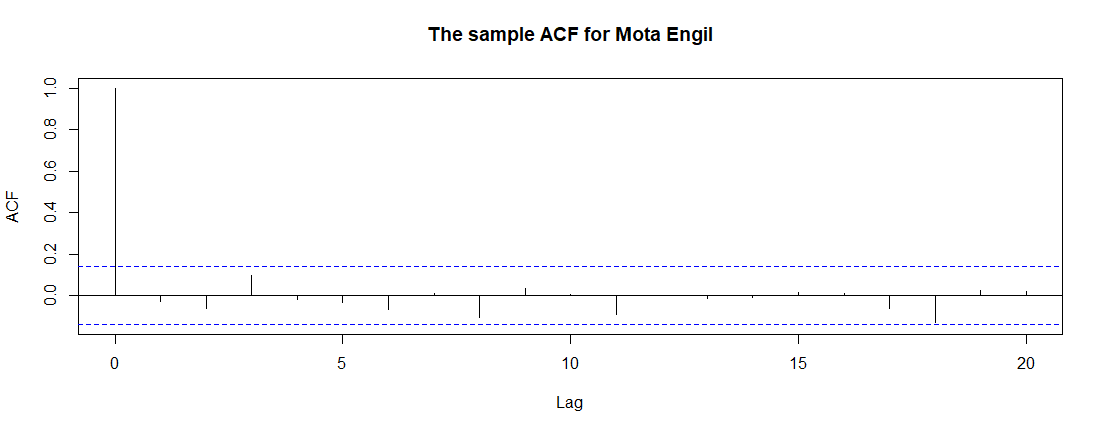
\includegraphics[width=0.45\textwidth]{Plots2/acf2.png}
   }
   \subfigure[The sample ACF for Ren.]{
   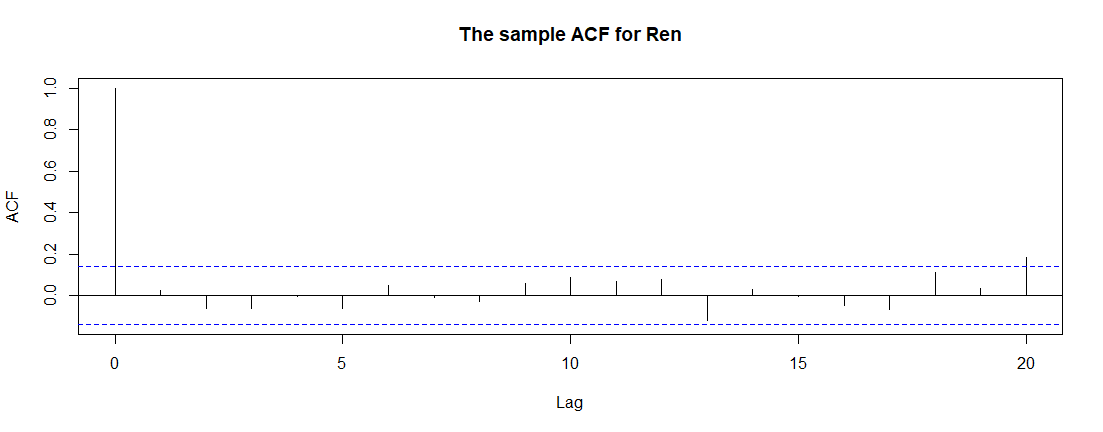
\includegraphics[width=0.45\textwidth]{Plots2/acf3.png}
   }
   \subfigure[The sample ACF for Sonae.]{
   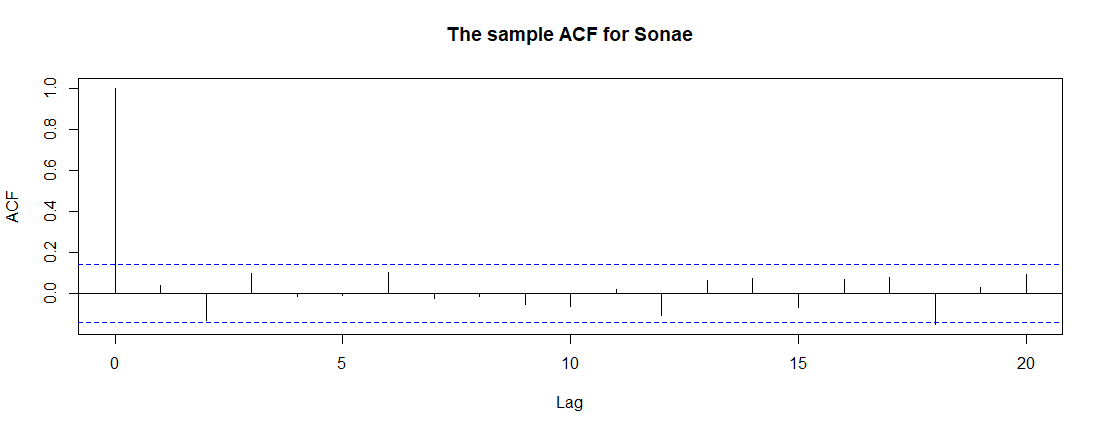
\includegraphics[width=0.45\textwidth]{Plots2/acf4.png}
   }
  \subfigure[The sample ACF for The Navigator Company.]{
   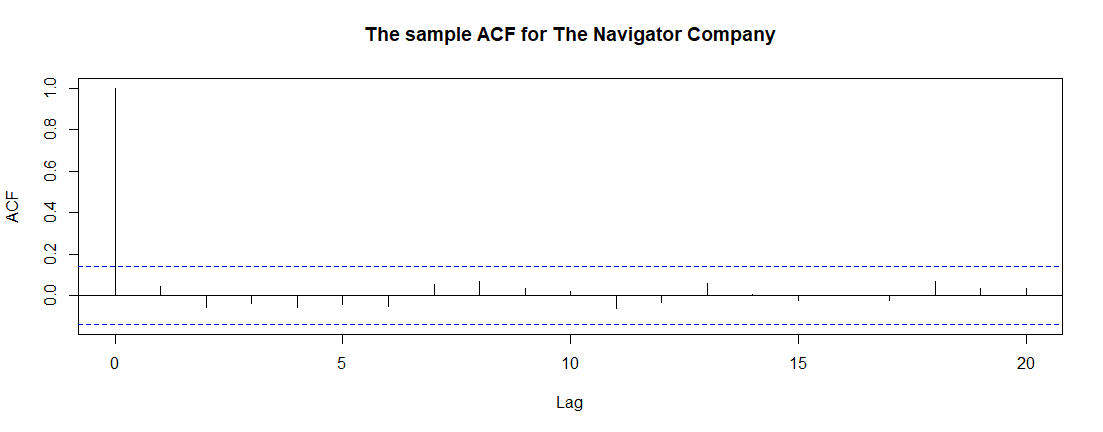
\includegraphics[width=0.45\textwidth]{Plots2/acf5.png}
   }
   \caption{The sample ACF for the five time series.}
    \label{fig:acf_lr}
\end{figure}

%\begin{figure}[ht!]
%   \centering
%   \subfigure[The sample ACF for the squares Altri-SGPS.]{
%   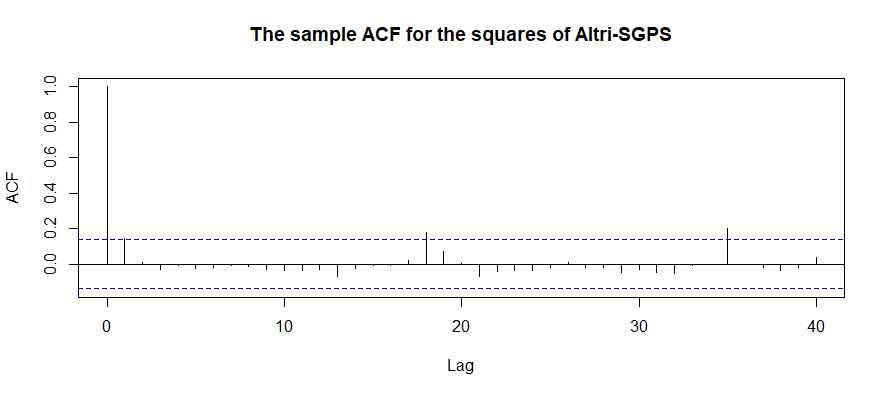
\includegraphics[width=0.45\textwidth]{Plots2/acf11.png}
%   }
%      \subfigure[The sample ACF for the squares Mota Engil.]{
%   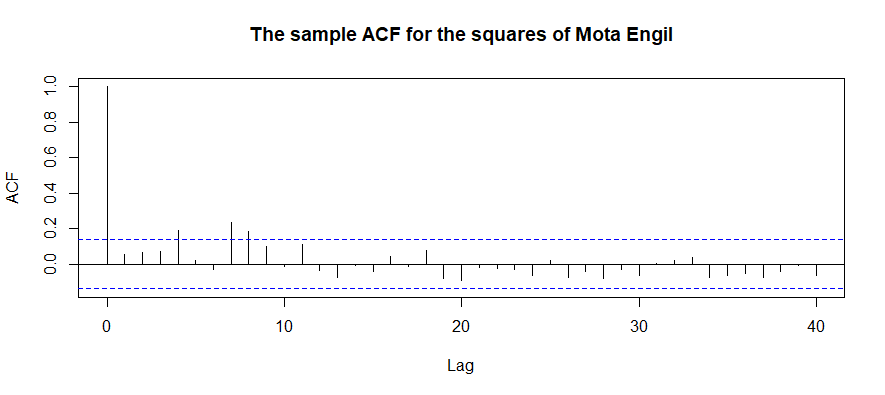
\includegraphics[width=0.45\textwidth]{Plots2/acf22.png}
%   }
%   \subfigure[The sample ACF for the squares Ren.]{
%   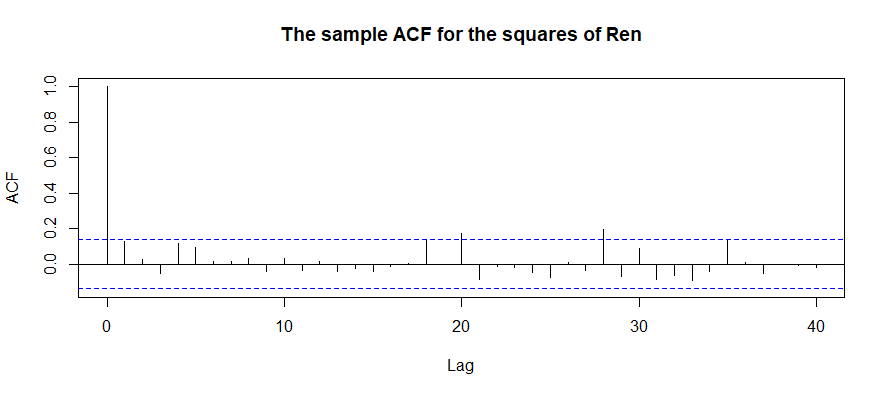
\includegraphics[width=0.45\textwidth]{Plots2/acf33.png}
%   }
%   \subfigure[The sample ACF  for the squares of Sonae.]{
%   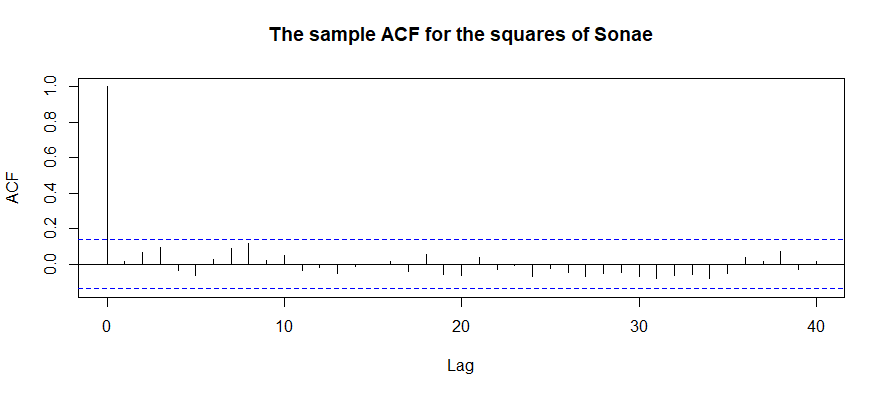
\includegraphics[width=0.45\textwidth]{Plots2/acf44.png}
%   }
%  \subfigure[The sample ACF for the squares of The Navigator Company.]{
%   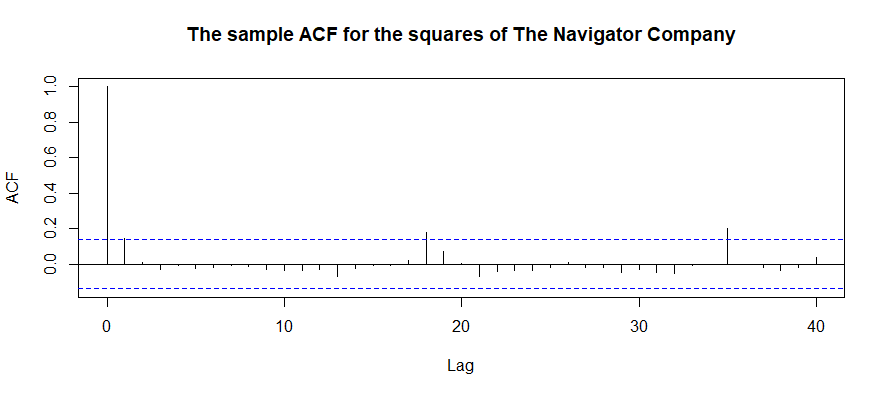
\includegraphics[width=0.45\textwidth]{Plots2/acf55.png}
%   }
%   \caption{The sample ACF for the squares of the five time series.}
%    \label{fig:acf_lr_sq}
%\end{figure}

\subsection{Model fitting}


In this subchapter I will discribe the step by step model fitting for the time series Altri-SGPS. From the sample ACF of the data we can see that the isn't any
linear dependence in the data.

We will start by an initial identification of the dependence orders. We will do this by firstly trying to fit a ARCH-type model to the time series. We fitted models \verb|ARCH(q)| for \verb|q = 1,2,3,4,5,6,7,8,9,10,15,20,40|. The model with the best AIC turned out to be  \verb|ARCH(3)|. The AIC value was -5.41. The $p$-value of $a_3$ in the model was 0.0156 indicating that it might be important for the final model. All of the other $a_i$ in this model (and most of the others) had very huge $p-$values indicating that thery might not be significantly influental.

Next we take a look at the \verb|GARCH(p,q)| models hoping to find a better one, where \verb|q = 1,2,3,4,5,6,7,8,9,10,15,20,40| and \verb|p = 1, 3|. The best model was  \verb|GARCH(3,1)| but with a larger AIC of  -5.40.

The next step we take is to try to fit a \verb|IGARCH(p, q)| model for the same choices of \verb|p| and \verb|q|, however the AIC of the best model is worst then the AIC of the best \verb|GARCH(p,q)| model.

Next we fit a \verb|GARCH-M(p, q)| model for the same choices of \verb|p| and \verb|q|, however the AIC of the best model is worst then the AIC of the best \verb|GARCH(p,q)| model. Model \verb|GARCH-M(1, 1)| had the best AIC of -5.37.

Finally we fit a \verb|APARCH(p, q)| model for the same choices of \verb|p| and \verb|q|. We find that the \verb|APARCH(1, 1)| model has the best AIC out of all of the mentioned models with an AIC of -5.46. The model has the parameter $\gamma = 1$ which indicates negative shocks have stronger impact on volatility than
positive shocks. This makes sence as we have noticed this in chapter \ref{sect:2.2}. 

For estimation of parameters we have used the packages \verb|fGarch| and \verb|rugarch|. 

\subsection{Residual diagnostics and model choice}

To select the final model we need to analyse  the residuals as well as model 
compare the models.

Let's firstly take a look at the the plot of the standardised residuals, their ACF and their Q-Q plot for the model with the lowest AIC, that being the \verb|APARCH(1, 1)| model. This can be seen in figure \ref{fig:aparch_rd}. From the figure it can be noted that the the standardized residuals follow an i.i.d. sequence with mean zero and variance one. If we take a closer look at the ACF there is not any patterns of large values. This statement is also supported by the Box-Ljung test with a $p-$value of 0.481.
Also on the Q-Q plot we see that the points lie along a straight line, indicating that they follow an i.i.d. sequence as stated before. Taking all this into account we can conclude that the model is a good fit for the given data.

\begin{figure}[ht!]
   \centering
         \subfigure[Plot of the standardised residuals for the model APARCH(1, 1).]{
   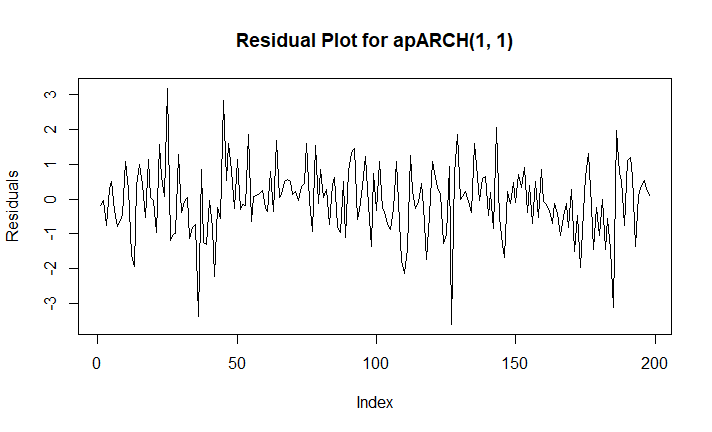
\includegraphics[width=0.45\textwidth]{Plots2/d_3.png}
   }

   \subfigure[The ACF function of the standardised residuals for the model APARCH(1, 1).]{
   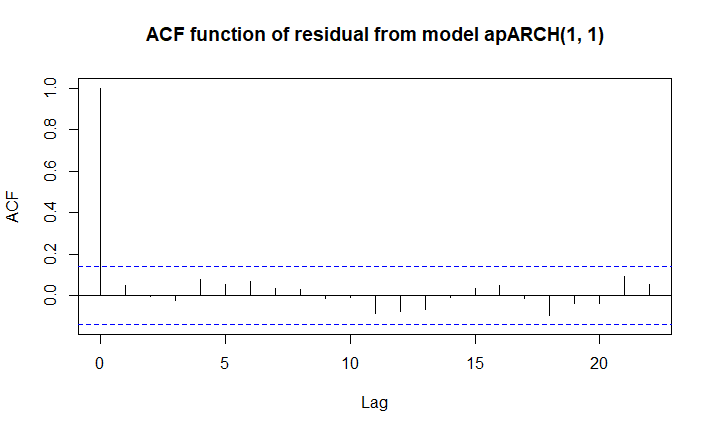
\includegraphics[width=0.45\textwidth]{Plots2/d_1.png}
   }
      \subfigure[Q-Q plot for the standardised residuals for the model APARCH(1, 1).]{
   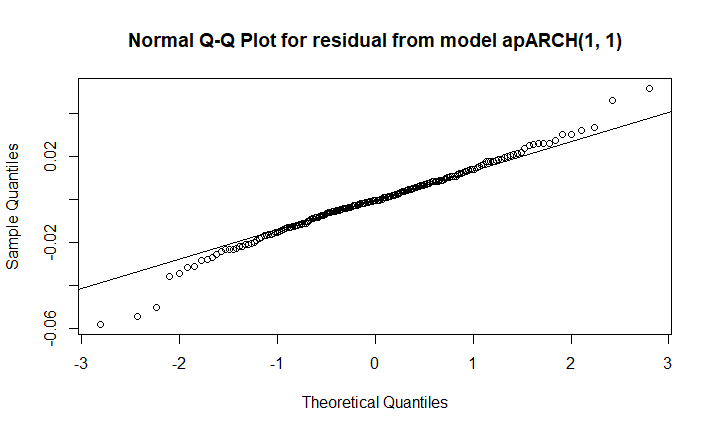
\includegraphics[width=0.45\textwidth]{Plots2/d_2.png}
   }
    \label{fig:aparch_rd}
\end{figure}

If we look at the same figures, on figure \ref{fig:aparch_rd2}, for second best model, that being the \verb|ARCH(3)| we see that the residuals also follow an i.i.d. sequence and appear to have no autocorrelation.

\begin{figure}[ht!]
   \centering
         \subfigure[Plot of the standardised residuals for the model ARCH(3).]{
   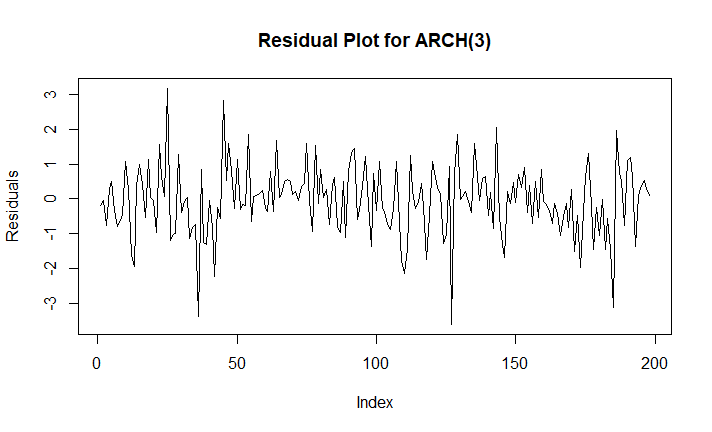
\includegraphics[width=0.45\textwidth]{Plots2/d_4.png}
   }

   \subfigure[The ACF function of the standardised residuals for the model ARCH(3).]{
   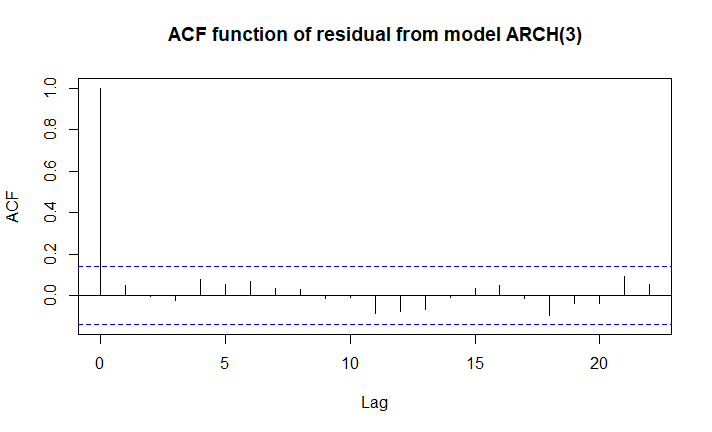
\includegraphics[width=0.45\textwidth]{Plots2/d_5.png}
   }
      \subfigure[Q-Q plot for the standardised residuals for the model ARCH(3).]{
   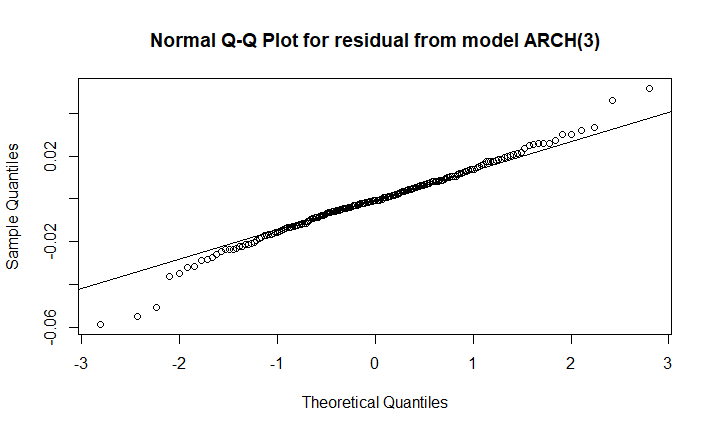
\includegraphics[width=0.45\textwidth]{Plots2/d_6.png}
   }
    \label{fig:aparch_rd2}
\end{figure}

For the other four time series we compleated the same exact procedure and the results of the respected models can be found in table 

\begin{table}[htbp]
  \centering
  \begin{tabular}{lccccc}
    \toprule
    \textbf{Model} & \textbf{Altri-SGPS} & \textbf{Mota Engil} & \textbf{Ren} & \textbf{Sonae} & \textbf{The Navigator Com.} \\
    \midrule
    \verb|ARCH(3)|& Value 1 & Value 2 & Value 3 & Value 4 & Value 5 \\ \hline 
    \verb|GARCH(3,1)|  & Value 6 & Value 7 & Value 8 & Value 9 & Value 10 \\ \hline
    \verb|GARCH-M(1,1)|  & Value 6 & Value 7 & Value 8 & Value 9 & Value 10 \\ \hline
    \verb|APARCH(1,1)|  & Value 6 & Value 7 & Value 8 & Value 9 & Value 10 \\ 
    \bottomrule
  \end{tabular}
  \caption{AIC of the fitted models for the financial time series of log returns.}
  \label{model:fs}
\end{table}




\appendix

\section{Appendix A}

\begin{table}
    \centering
    \begin{tabular}{|l|c|c|}
    \toprule
    \textbf{Model} & \textbf{AIC} & \textbf{RMSE} \\
    \midrule 
    SARIMA$(0,1,0) \times (1,1,0)_{24}$ & 60454 & 7.7 \\
    SARIMA$(0,0,0) \times (1,0,0)_{24}$ & 75627 & 18.1 \\
    SARIMA$(5,1,0) \times (2,0,0)_{24}$ & 58194 & 6.7 \\
    SARIMA$(1,0,1) \times (2,1,0)_{24}$ & 58874 & 7.0 \\
    SARIMA$(3,0,1) \times (1,0,1)_{24}$ & 57103 & 6.2 \\
    SARIMA$(3,0,0) \times (1,0,0)_{24}$ & 58032 & 6.6 \\
    SARIMA$(1,0,1) \times (1,0,1)_{24}$ & 57103 & 6.3 \\
    SARIMA$(2,0,1) \times (1,1,1)_{24}$ & 56962 & 6.3 \\
    SARIMA$(2,1,1) \times (1,1,1)_{24}$ & 56962 & 6.3 \\
    SARIMA$(1,0,1) \times (1,0,2)_{24}$ & 57426 & 6.4 \\
    \bottomrule
    \end{tabular}
    \caption{AIC and RMSE of the fitted models for the Reboleira ozon-ground level time series.}
    \label{tab:Reboleira}
\end{table}

\begin{table}
    \centering
    \begin{tabular}{|l|c|c|}
    \toprule
    \textbf{Model} & \textbf{AIC} & \textbf{RMSE} \\
    \midrule 
    SARIMA$(0,1,0) \times (1,1,0)_{24}$ & 60659 & 7.8 \\
    SARIMA$(0,0,0) \times (1,0,0)_{24}$ & 75269 & 17.7  \\
    SARIMA$(5,1,0) \times (2,0,0)_{24}$ & 58699 & 6.9 \\
    SARIMA$(1,0,1) \times (2,1,0)_{24}$ & 59222 & 7.2 \\
    SARIMA$(3,0,1) \times (1,0,1)_{24}$ & 57481 & 6.4 \\
    SARIMA$(3,0,0) \times (1,0,0)_{24}$ & 58515 & 6.8 \\
    SARIMA$(1,0,1) \times (1,0,1)_{24}$ & 57499 & 6.4 \\
    SARIMA$(2,0,1) \times (1,1,1)_{24}$ & 57313 & 6.4 \\
    SARIMA$(2,1,1) \times (1,1,1)_{24}$ & 57361 & 6.4 \\
    SARIMA$(1,0,1) \times (1,0,2)_{24}$ & 57432 & 6.4 \\
    \bottomrule
    \end{tabular}
    \caption{AIC and RMSE of the fitted models for the Beato ozon-ground level time series.}
    \label{tab:Beato}
\end{table}

\begin{table}
    \centering
    \begin{tabular}{|l|c|c|}
    \toprule
    \textbf{Model} & \textbf{AIC} & \textbf{RMSE} \\
    \midrule 
    SARIMA$(0,1,0) \times (1,1,0)_{24}$ & 63969 & 9.4 \\
    SARIMA$(0,0,0) \times (1,0,0)_{24}$ & 77832 & 20.5 \\
    SARIMA$(5,1,0) \times (2,0,0)_{24}$ &  61938 & 8.3 \\
    SARIMA$(1,0,1) \times (2,1,0)_{24}$ & 62386 & 8.5  \\
    SARIMA$(3,0,1) \times (1,0,1)_{24}$ & 60603 & 7.6 \\
    SARIMA$(3,0,0) \times (1,0,0)_{24}$ & 61763 & 8.2  \\
    SARIMA$(1,0,1) \times (1,0,1)_{24}$ & 60610 & 7.7 \\
    SARIMA$(2,0,1) \times (1,1,1)_{24}$ & 60454 & 7.6 \\
    SARIMA$(2,1,1) \times (1,1,1)_{24}$ & 60501 & 7.7 \\
    SARIMA$(1,0,1) \times (1,0,2)_{24}$ &  60584 & 7.7 \\
    \bottomrule
    \end{tabular}
    \caption{AIC and RMSE of the fitted models for the Olivais ozon-ground level time series.}
    \label{tab:Olivais}
\end{table}

\begin{table}
    \centering
    \begin{tabular}{|l|c|c|}
    \toprule
    \textbf{Model} & \textbf{AIC} & \textbf{RMSE} \\
    \midrule 
    SARIMA$(0,1,0) \times (1,1,0)_{24}$ & 63315.33 & 9.1  \\
    SARIMA$(0,0,0) \times (1,0,0)_{24}$ & 77183 & 19.8   \\
    SARIMA$(5,1,0) \times (2,0,0)_{24}$ & 61160 & 7.9  \\
    SARIMA$(1,0,1) \times (2,1,0)_{24}$ & 61748 & 8.2   \\
    SARIMA$(3,0,1) \times (1,0,1)_{24}$ & 60017 & 7.4  \\
    SARIMA$(3,0,0) \times (1,0,0)_{24}$ & 61063 & 7.9   \\
    SARIMA$(1,0,1) \times (1,0,1)_{24}$ & 59811 & 7.4  \\
    SARIMA$(2,0,1) \times (1,1,1)_{24}$ & 59902 & 7.4  \\
    SARIMA$(2,1,1) \times (1,1,1)_{24}$ & 59918 & 7.4  \\
    SARIMA$(1,0,1) \times (1,0,2)_{24}$ & 60012 & 7.4  \\
    \bottomrule
    \end{tabular}
    \caption{AIC and RMSE of the fitted models for the Entrecampos ozon-ground level time series.}
    \label{tab:Entrecampos}
\end{table}


\newpage

\begin{thebibliography}{99}
   \bibitem{i1}
   \emph{Ground-Level Ozone (O3) Pollution}
   [viewed 31.~05.~2023], can be found at 
   \url{https://www.azdeq.gov/ground-level-ozone-o3-pollution} 
   \bibitem{i2}
    \emph{Qualar}
   [viewed 31.~05.~2023], can be found at 
   \url{https://qualar.apambiente.pt/} 
   \bibitem{i3}
   \emph{Which blood pressure number is important?}
   [viewed 28.~05.~2023], can be found at   
   \url{https://www.health.harvard.edu/staying-healthy/which-blood-pressure-number-is-important} 
   \bibitem{i4}
   The Seventh Report of the Joint National Committee on Prevention, Detection, Evaluation, and Treatment of High Blood Pressure (2003 Guideline)
   \bibitem{i5}
   M. Sue Kirkman, Vanessa Jones Briscoe, Nathaniel Clark, Hermes Florez, Linda B. Haas, Jeffrey B. Halter, Elbert S. Huang, Mary T. Korytkowski, Medha N. Munshi, Peggy Soule Odegard, Richard E. Pratley, Carrie S. Swift; Diabetes in Older Adults. Diabetes Care 1 December 2012; 35 (12): 2650–2664
   \bibitem{i6}
   Schorling JB, Roach J, Siegel M, Baturka N, Hunt DE, Guterbock TM, Stewart HL (1997) A trial of church-based smoking cessation interventions for rural African Americans. Preventive Medicine 26:92-101.
   \bibitem{i7}
   \emph{Body Frame Size Measuring Tables}
   [viewed 28.~05.~2023], can be found at   
   \url{https://www.disabled-world.com/calculators-charts/body-frame.php}
    \bibitem{i8}
    Silva, G.L. (2023). Lecture Notes of Biostatistics. Lisbon, Instituto Superior Tecnico
    \bibitem{i9}
   \emph{Blood Glucose (Sugar) Test}
   [viewed 28.~05.~2023], can be found at       
    \url{https://my.clevelandclinic.org/health/diagnostics/12363-blood-glucose-test}
    \bibitem{i10}
    \emph{What is Diabetes?}
   [viewed 28.~05.~2023], can be found at       
    \url{https://www.cdc.gov/diabetes/basics/diabetes.html}

\end{thebibliography}

\end{document}



